\documentclass[11pt]{article}
\usepackage[margin=1in]{geometry}
\usepackage[T1]{fontenc}
\usepackage[utf8]{inputenc}
\usepackage{lmodern}
\usepackage{microtype}
\usepackage{amsmath,amssymb,amsthm}
\usepackage{graphicx}
\usepackage{booktabs,tabularx,array}
\usepackage{xcolor}
\usepackage[numbers,sort&compress]{natbib}
\usepackage{tikz}
\usetikzlibrary{arrows.meta,positioning}
\usepackage{enumitem}
\usepackage[hidelinks]{hyperref}
\usepackage[capitalise,noabbrev]{cleveref}
\usepackage{draftwatermark}
\DraftwatermarkOptions{text=DRAFT, color=black!12, fontsize=3.5cm, angle=45}

\definecolor{notecolor}{HTML}{C2410C}
\newcommand{\note}[1]{\textcolor{notecolor}{\small[\textbf{Note:} #1]}}

\theoremstyle{plain}
\newtheorem{theorem}{Theorem}
\newtheorem{proposition}{Proposition}
\newtheorem{lemma}{Lemma}
\newtheorem{corollary}{Corollary}
\theoremstyle{definition}
\newtheorem{definition}{Definition}
\theoremstyle{remark}
\newtheorem{remark}{Remark}

\newcommand{\E}{\mathbb{E}}
\newcommand{\R}{\mathbb{R}}
\newcommand{\abar}{\bar a}
\newcommand{\Pbar}{\bar P}
\newcommand{\eps}{\varepsilon}

\title{\textbf{Types of Intelligence:}\\[2pt]
\Large Adaptation Spectra, Consolidation, and the Partial Order of Minds}
\author{Asim Imdad Wagan\thanks{AKS iQ. Correspondence: \texttt{dr.asim@aksiq.com}. Code and \LaTeX{} sources: \url{https://github.com/drasimwagan/aitypes}.}}
\date{Working draft v0.2 --- \today\\[4pt]
\small\textit{Draft for comment. Comments and criticism are very welcome; please do not cite without contacting the author.}}

\begin{document}
\maketitle

\begin{abstract}
Debates about whether artificial intelligence is ``smarter'' than humans presuppose that intelligence is a scalar. We argue that it is not, and we propose a formal framework in which kinds of intelligence are distinguished by the \emph{temporal structure} of their adaptation. Any adaptive system is modelled as a hierarchy of state variables updated and erased on different timescales. A system is then characterised by a profile: its \emph{adaptation spectrum} (what it can learn at each timescale), its \emph{consolidation coefficients} (how much of what is learned quickly survives into slow memory), its \emph{instance topology} (how many bodies read from and write to one slow memory), its \emph{goal horizon}, and its \emph{embodiment}. On this view, the salient difference between humans and today's deployed language models is not that one learns in real time and the other does not---both adapt within an episode---but that humans consolidate within-lifetime experience into long-term memory, whereas deployed models do not: their learning happens at the level of the \emph{lineage}, in batches, with a lag. In a minimal, exactly solvable model of episodic tracking in a drifting world, we prove that a consolidating individual and an amnesic but vastly more experienced lineage are \emph{incomparable}: each is strictly better in worlds that drift at different rates. The crossover drift rate scales with the inverse square of the lineage's staleness and saturates in the amount of pooled experience, so more data cannot substitute for consolidation. A ``hive'' learner that consolidates continuously across many instances dominates both. Intelligence is therefore a partial order, and any scalar measure implicitly chooses which timescales matter. We use the framework to enumerate forms of intelligence that biology could not have produced, because evolution builds cognitive capacities cumulatively while engineering can recombine them.
\end{abstract}

% =====================================================================
\section{Introduction}
\label{sec:intro}

There is an intuitive ladder of intelligence. Inert matter has no goals. Viruses and bacteria respond to their surroundings; animals of increasing size and neural complexity learn, plan and communicate; humans build cumulative culture; and artificial systems now converse, write code and solve competition mathematics. Somewhere along this ladder ``will'' appears, and somewhere near its top the question arises whether machines have overtaken us.

The ladder is a useful starting point and a misleading end point. It is misleading in two ways. First, it projects a space of many dimensions onto one, inviting the old \emph{scala naturae} error of ranking organisms that are adapted to different problems. Second, it hides the feature that most sharply separates current artificial systems from animals: not how much they know, nor how fast they compute, but \emph{when and where they learn}.

A common way of stating the human--AI contrast is that humans ``update the model in real time'' while AI systems are trained once and then only perform inference. This is close to right but, as stated, it is wrong in both directions. Humans do not fully update in real time: much of what is learned during the day is consolidated offline, from hippocampus to neocortex, during sleep~\citep{mcclelland1995why,diekelmann2010memory}, and many priors are not revisable at all. Deployed language models, conversely, \emph{do} adapt in real time: in-context learning changes a fast internal state in response to evidence, and can implement learning algorithms in its forward pass~\citep{brown2020language,garg2022what,vonoswald2023transformers}. The real difference is what happens to fast learning \emph{afterwards}. In humans a fraction of it is written into slow memory. In a deployed model the context is erased at the end of the episode; experience reaches the weights, if at all, only when logged interactions feed a later training run, months later. A deployed model is in this respect like the amnesic patient H.M.~\citep{scoville1957loss}: intact knowledge, intact working memory, and no new long-term memories---an analogy that has also been drawn by researchers working on continual learning~\citep{behrouz2025nested}.

This reframing has a consequence that we think is underappreciated. Because learning in a deployed model occurs across releases rather than within an instance, a model family is structurally more like a \emph{species} than like an individual: the weights play the role of a genome plus inherited culture, and each conversation is a lifetime that passes nothing on except through the lineage. Biological minds acquired their capacities cumulatively---every animal that can learn from consequences also evolves, and every animal that thinks with cultural tools also learns from consequences~\citep{dennett1995darwin,dennett1996kinds}. Engineered minds need not. Current models have the ``top floors'' of Dennett's tower of generate-and-test (they are built almost entirely from language and culture, and can deliberate before acting) while lacking one of the lower floors (they do not learn from the consequences of their own actions during deployment). Our central thesis is that \emph{evolution builds intelligences cumulatively, whereas engineering can build them combinatorially}, and that the space of possible minds is correspondingly larger than the biological ladder suggests.

\paragraph{Contributions.}
\begin{enumerate}[leftmargin=*,itemsep=2pt]
\item A framework that describes any adaptive system---from a bacterium to a civilisation to a language model---as a hierarchy of states with characteristic update and erasure times, summarised by a profile $\Phi(S)$ (\cref{sec:framework}).
\item A reformulation of the human--AI contrast in terms of consolidation and instance topology rather than ``real-time learning'', with the species analogy and the decoupling of Dennett's tower as corollaries (\cref{sec:reading}).
\item A minimal, exactly solvable model in which we prove that intelligence is only partially ordered: a consolidating individual and an amnesic lineage are incomparable, a hive learner dominates both, and the crossover drift rate obeys a simple scaling law that saturates in experience (\cref{sec:model}).
\item A generative taxonomy of possible intelligences obtained by varying the profile's components independently, including forms with no biological counterpart (\cref{sec:space}).
\end{enumerate}

% =====================================================================
\section{From matter to minds: what actually varies}
\label{sec:ladder}

\paragraph{Where goal-directedness begins.}
William James distinguished iron filings drawn to a magnet from Romeo drawn to Juliet: put a card between filings and magnet and the filings press against it forever; put a wall between the lovers and Romeo climbs it~\citep{james1890principles}. The difference is not the presence of an end state but the \emph{variability of means under perturbation}. Following \citet{rosenblueth1943behavior} we take this counterfactual compensation as the operational mark of goal-directedness. Matter that merely relaxes to an equilibrium does not compensate; a chemotactic bacterium does, over micrometres and seconds; a human does, over years and continents. The \emph{extent} of compensation in space and time is what \citet{levin2019computational,levin2022tame} calls the cognitive light cone. It is one axis of our profile, not the only one.

\paragraph{The ladder as a projection.}
The intuitive ladder conflates at least five quantities that vary independently: the timescales on which a system can absorb information; whether fast learning is retained; how many bodies share one memory; how far its goals extend; and how strongly it can act on its world. Colonies of ants, immune systems and slime moulds solve problems without any fixed wiring~\citep{sole2019liquid,nakagaki2000maze}; bacteria with CRISPR systems write a record of past infections into their genome~\citep{barrangou2007crispr}; human culture accumulates knowledge over centuries through a ``ratchet'' that no individual could reproduce~\citep{tomasello1999cultural,boyd1985culture,henrich2016secret}. None of these sits at a single point on a line.

\paragraph{Towers and trees.}
\citet{dennett1995darwin,dennett1996kinds} ordered minds by where trial and error happens: \emph{Darwinian} creatures learn only by selection across generations; \emph{Skinnerian} creatures also learn from the consequences of their own actions; \emph{Popperian} creatures pre-select actions by simulating them internally; \emph{Gregorian} creatures think with cultural tools such as language. \citet{godfreysmith2018towers} argued that only the lower floors form a nested tower and that the upper capacities form a branching tree. Our point is complementary and concerns artificial systems: in biology every known Gregorian creature is also Skinnerian, because the capacities were acquired in sequence. Engineered systems break this constraint. A deployed language model is Gregorian and, with deliberate reasoning, Popperian, yet in deployment it is not Skinnerian: nothing it experiences changes its long-term dispositions. This configuration is not a point on the biological ladder at all.

% =====================================================================
\section{A framework: adaptive systems as multi-timescale hierarchies}
\label{sec:framework}

We describe a system by the timescales on which its internal state changes and by what flows between those timescales. Throughout, time is discrete, $t\in\mathbb{N}$, and the system interacts with an environment $\mu$ through observations $o_t$ and actions $a_t$.

\begin{definition}[Multi-timescale adaptive system]
\label{def:mtas}
An adaptive system is a tuple
\[
S=\big(\{Z_k,\tau_k,\sigma_k,U_k\}_{k=1}^{K},\;\pi\big)
\]
in which level $k$ has state $z_k\in Z_k$, update period $\tau_k$ (with $\tau_1\le\dots\le\tau_K$), and erasure period $\sigma_k\in\mathbb{N}\cup\{\infty\}$: every $\tau_k$ steps the state is updated,
\[
z_k\leftarrow U_k(z_k,\,z_{k-1},\,z_{k+1}),
\]
with $z_0$ the observation stream, and every $\sigma_k$ steps it is reset to a default $z_k^{0}$. Actions are drawn from a policy $\pi(a_t\mid o_t,z_1,\dots,z_K)$.
\end{definition}

For a human, levels range from neural activity (milliseconds) through working memory (seconds), hippocampal traces consolidated during sleep (hours to days), and skills and semantic knowledge (months to a lifetime), to culture and genes (generations). For a deployed language model they are the activations of a forward pass (milliseconds), the context (one conversation, erased when it ends), and the weights (changed only by training runs). \Cref{fig:spectra} sketches these hierarchies.

\begin{figure}[t]
\centering
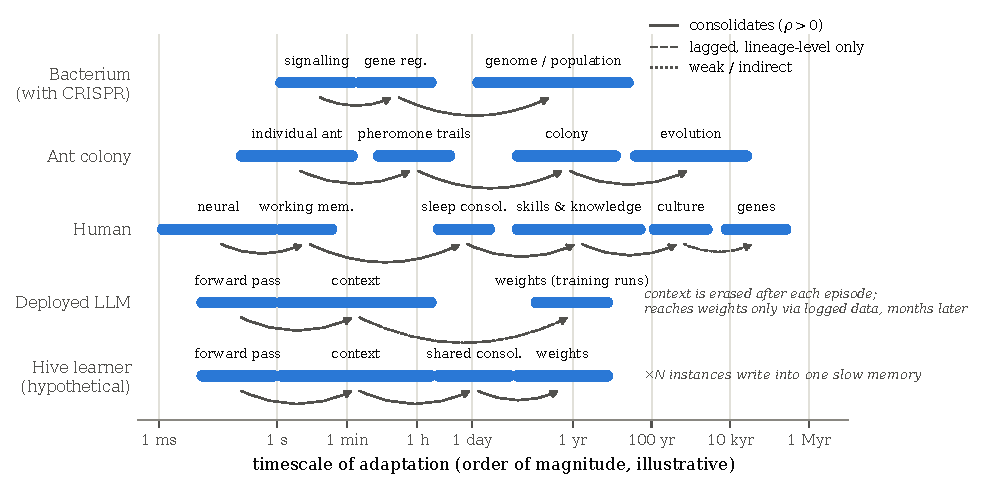
\includegraphics[width=\linewidth]{figures/fig_spectra.pdf}
\caption{\textbf{Adaptation spectra.} Each bar is a level of state that changes on the indicated timescale (orders of magnitude, illustrative). Arrows show whether information learned at one level is written into the next (\emph{consolidation}). In a deployed language model the context is erased after each episode and reaches the weights only through logged data used in a later training run; a hypothetical hive learner consolidates continuously from many instances into one slow memory.}
\label{fig:spectra}
\end{figure}

\begin{definition}[Adaptation spectrum]
The capacity of level $k$ is $B_k=\sup I\big(z_k(t+\tau_k);\,x_{(t,t+\tau_k]}\,\big|\,z_k(t)\big)$, the largest amount of information about new experience $x$ that one update can absorb, the supremum being over experience distributions. The adaptation spectrum is $\mathcal{A}(S)=\{(\tau_k,\sigma_k,B_k)\}_{k=1}^K$.
\end{definition}

\begin{definition}[Consolidation and retention]
\label{def:consolidation}
Let $\theta$ be a task-relevant feature of the world and let $\mathcal{I}_k$ denote the Fisher information about $\theta$ held at level $k$ just before an erasure. The \emph{consolidation coefficient} of level $k$ is
\[
\rho_k=\frac{\mathcal{I}_{k+1}^{\,\mathrm{gain}}}{\mathcal{I}_k}\in[0,1],
\]
the fraction of that information which level $k+1$ has gained from level $k$ by the time level $k$ is erased. More generally, the \emph{retention function} $R_S(\Delta)$ is the fraction of the information about a window of experience that the whole system still carries $\Delta$ steps later---an Ebbinghaus curve~\citep{ebbinghaus1885gedachtnis} for arbitrary systems.
\end{definition}

The Fisher-information form is convenient because information about a parameter from independent sources adds; in a Bayesian setting, retaining a fraction $\rho$ of an episode's information is equivalent to a power prior with exponent $\rho$~\citep{ibrahim2000power}. For a deployed language model, $\rho_{\text{context}\to\text{weights}}\approx0$ at the level of the instance, and $R_S(\Delta)$ drops to zero when the context is erased.

\begin{definition}[Instance topology]
The instance topology $\mathcal{G}(S)$ is a directed graph whose nodes are the levels of all running instances and whose edges are \emph{write} edges (consolidation from a fast level into a slow one) and \emph{read} edges (initialisation of an instance from a slow level). Its summary statistics include the number $N_k$ of instances that read from a level-$k$ memory, the number that write to it, and the lag of each write edge. Copying, pausing, resetting, forking and merging are operations on $\mathcal{G}$.
\end{definition}

A human has $N=1$ at every individual level; culture is a slow level with very many writers and a lag of years. A deployed model has thousands of instances reading from one set of weights and, during deployment, none writing to it. An ant colony has many simple instances writing to a shared, rapidly decaying memory (pheromone trails).

\begin{definition}[Goal horizon and embodiment]
A system is goal-directed toward a set of world states $G$ with respect to a class of perturbations $\mathcal{D}$ if, for perturbations in $\mathcal{D}$, its trajectories still reach $G$ by means that vary with the perturbation~\citep{james1890principles,rosenblueth1943behavior}. The \emph{goal horizon} $H=(H_{\mathrm{space}},H_{\mathrm{time}})$ is the largest spatial region and time span over which the system compensates in this way---the cognitive light cone of \citet{levin2019computational}. \emph{Embodiment} $E$ is measured by empowerment, $E_n=\max_{p(a_{t:t+n})} I(a_{t:t+n};o_{t+n})$, the capacity of the action--perception channel~\citep{klyubin2005empowerment}.
\end{definition}

\begin{definition}[Profile]
The profile of $S$ is $\Phi(S)=\big\langle\mathcal{A}(S),\,\{\rho_k\},\,\mathcal{G}(S),\,H,\,E\big\rangle$.
\end{definition}

Profiles are descriptive. To compare systems we need performance, and performance depends on the environment.

\begin{definition}[Dominance]
\label{def:dominance}
Let $\mathcal{E}$ be a family of environments and $V_\mu(S)$ the expected performance of $S$ in $\mu\in\mathcal{E}$. $S$ \emph{dominates} $S'$ on $\mathcal{E}$, written $S\succeq_{\mathcal{E}}S'$, if $V_\mu(S)\ge V_\mu(S')$ for every $\mu\in\mathcal{E}$. Two systems are \emph{incomparable} if neither dominates.
\end{definition}

Dominance is a preorder. A scalar measure such as universal intelligence~\citep{legg2007universal}, $\Upsilon_w(S)=\sum_{\mu}w(\mu)V_\mu(S)$ with $w(\mu)=2^{-K(\mu)}$, is monotone with respect to $\succeq$, but whenever two systems are incomparable their scalar ranking depends on the weighting $w$. The substantive question is therefore whether incomparability actually arises between systems we care about. \Cref{sec:model} shows that it does, for the pair that motivates this paper.

\subsection{Reading the profiles: humans and deployed language models}
\label{sec:reading}

\Cref{tab:profiles} applies the framework qualitatively. Four observations follow.

\emph{Both adapt in real time.} The fast levels of humans and models both change within seconds in response to evidence; in-context learning is genuine adaptation~\citep{vonoswald2023transformers}.

\emph{They differ in erasure and consolidation.} The model's context has a finite erasure period and $\rho\approx0$ into the weights during deployment; the human's working memory is also erased, but a fraction is consolidated~\citep{mcclelland1995why,kumaran2016what}.

\emph{Learning happens in different places.} For the model, the write edge into slow memory runs from the population of instances to the next training run, with a lag of months. The unit that learns is the lineage, as in a species; the unit that acts is the instance, as in an organism.

\emph{``Scale'' is several quantities.} Models are not larger in parameters: the human brain has about $8.6\times10^{10}$ neurons~\citep{azevedo2009equal} and on the order of $10^{14}$ synapses, whereas frontier models are believed to have on the order of $10^{12}$ parameters (most counts are undisclosed). They are larger in \emph{experience}---trained on more than $10^{13}$ tokens~\citep{grattafiori2024llama}, against roughly $10^{8}$ words heard by a 20-year-old, a gap of three to five orders of magnitude~\citep{frank2023bridging}---and in \emph{copyability}.

\begin{table}[t]
\centering
\small
\renewcommand{\arraystretch}{1.15}
\begin{tabularx}{\linewidth}{@{}>{\raggedright}p{2.3cm}>{\raggedright}X>{\raggedright}p{2.4cm}>{\raggedright}p{2.6cm}>{\raggedright\arraybackslash}p{2.4cm}@{}}
\toprule
System & Levels (fast $\to$ slow) & Consolidation & Instance topology & Goal horizon \\
\midrule
Thermostat & one fixed set-point & none & 1 & local, immediate \\
Bacterium & signalling; gene regulation; genome & genome via selection; CRISPR & populations of clones & $\mu$m--mm, seconds \\
Ant colony & ant; pheromone field; colony; genome & trails decay; colony learns & many writers, shared field & territory, seasons \\
Human & neural; working memory; episodic; semantic; culture; genes & sleep consolidation; teaching & 1 per mind; culture shared & years, communities \\
Deployed LLM & activations; context; weights & none in deployment; lineage via logged data & thousands read, none write & one task or conversation \\
LLM + memory tools & activations; context; external store; weights & into external store & per user or shared & longer, task-bound \\
Evolution & genomes; populations & selection & all organisms & none (no goals) \\
\bottomrule
\end{tabularx}
\caption{\textbf{Qualitative profiles.} Embodiment is omitted for space. Entries are indicative and intended to show that the components vary independently. \note{refine with references per row}}
\label{tab:profiles}
\end{table}

% =====================================================================
\section{A minimal model: amnesic lineages versus consolidating individuals}
\label{sec:model}

We now isolate the consolidation and topology components in a model simple enough to solve exactly. Goal horizon and embodiment are held fixed; every agent has the same fast level (in-context learning that is Bayes-optimal within an episode) and the agents differ \emph{only} in how their slow memory is formed.

\subsection{Environment}
A slow, shared feature of the world drifts as a random walk,
\begin{equation}
g_{e+1}=g_e+w_e,\qquad w_e\sim\mathcal{N}(0,Q),
\end{equation}
where $e$ indexes episodes (conversations, days) and $Q\ge0$ is the drift rate. Instances $i=1,\dots,N$ run concurrently. In episode $e$, instance $i$ faces a situation-specific offset $\ell_{e,i}\sim\mathcal{N}(0,s^2)$ and observes
\begin{equation}
y_{e,i,n}=u_{e,i}+v_{e,i,n},\qquad u_{e,i}=g_e+\ell_{e,i},\quad v\sim\mathcal{N}(0,r),\quad n=1,\dots,L.
\end{equation}
Before each observation the agent predicts it; since $\E(y-\hat y)^2=r+\E(u-\hat y)^2$, we score the \emph{excess loss} $\eps=\frac1L\sum_n\E(u-\hat y_n)^2$. All noise terms are independent. A single episode's data carry information about $g_e$ only through the episode mean, $\bar y_{e,i}\sim\mathcal{N}(g_e,\sigma^2)$ with
\begin{equation}
\sigma^2=s^2+r/L
\end{equation}
(\Cref{lem:suff} in \cref{app:proofs}).

\subsection{Agents}
Every agent enters an episode with a Gaussian belief $\mathcal{N}(m,P)$ about $g_e$---its slow memory---and then updates its belief about $u$ by exact Bayesian inference as observations arrive. Slow memory is \emph{calibrated}: $g_e-m\sim\mathcal{N}(0,P)$. Consolidation with retention $\rho\in(0,1]$ passes the episode statistic through a Gaussian channel, $z=\bar y+\eta$ with $\eta\sim\mathcal{N}\big(0,\sigma^2(\rho^{-1}-1)\big)$, so that a fraction $\rho$ of the episode's Fisher information about $g$ is retained (\cref{def:consolidation}). Slow memories are Kalman filters~\citep{kalman1960new} over these consolidated statistics.

\begin{description}[leftmargin=0.5cm,itemsep=2pt,font=\normalfont\itshape]
\item[Consolidating individual (human-like).] $N=1$; after each episode, consolidates its own experience with retention $\rho$.
\item[Hive learner.] $N$ instances share one slow memory, and each consolidates into it after every episode with retention $\rho$.
\item[Amnesic lineage (LLM-like).] $N$ instances never consolidate during deployment. A training process pools all instances' logged episodes with retention $\rho_L$; a snapshot is cut every $\tau$ episodes and deployed after a lag of $\Lambda$ episodes, then used for the next $\tau$ episodes. Its mean staleness is $\abar=\Lambda+(\tau+1)/2$ episodes.
\item[Darwinian lineage.] As the amnesic lineage, but with no fast level: it predicts its prior mean throughout the episode.
\end{description}

\subsection{Results}
All proofs are in \cref{app:proofs}. The first result reduces performance to a single number per episode: how uncertain the slow memory is when the episode begins.

\begin{proposition}[Reduction]
\label{prop:reduction}
An agent entering an episode with calibrated slow memory $\mathcal{N}(m,P)$ incurs expected excess loss
\begin{equation}
f(P)=\frac1L\sum_{n=0}^{L-1}\Big[\frac{1}{P+s^2}+\frac{n}{r}\Big]^{-1},
\label{eq:f}
\end{equation}
which is strictly increasing and concave in $P$, with $f(P)=(P+s^2)/L+\frac1L\sum_{n=1}^{L-1}r/n+o(1)$ as $P\to\infty$.
\end{proposition}

\begin{proposition}[Steady states]
\label{prop:steady}
Let $\Pbar(x)=\tfrac12\big[Q+\sqrt{Q^2+4Q\sigma^2/x}\big]$, the stationary prior variance of a Kalman filter that receives $x$ units of episode evidence per step. In steady state,
\begin{align}
\eps_{\mathrm{ind}}&=f\big(\Pbar(\rho)\big), \qquad \eps_{\mathrm{hive}}=f\big(\Pbar(N\rho)\big),\\
\eps_{\mathrm{lin}}&=\frac1\tau\sum_{j=1}^{\tau}f\big(P_j\big),\qquad \eps_{\mathrm{dar}}=\frac1\tau\sum_{j=1}^{\tau}\big(P_j+s^2\big),\qquad P_j=\Pbar(N\rho_L)+(\Lambda+j-1)Q.
\end{align}
$\Pbar(x)$ is strictly decreasing in $x$; $\Pbar(x)=\sqrt{Q\sigma^2/x}+Q/2+O(Q^{3/2})$ as $Q\to0$, and $\Pbar(x)\le Q+\sigma^2/x$.
\end{proposition}

The amnesic lineage pays twice for its structure: its prior is as good as $N\rho_L$ units of evidence per episode can make it, but it is $\Lambda+j$ episodes out of date. The individual has far less evidence but is never out of date.

\begin{theorem}[Incomparability]
\label{thm:incomparable}
Suppose $N\rho_L>\rho$ (the lineage pools more evidence than the individual retains) and $\abar>1$ (the lineage is not continuously updated). Then there exist $0<Q_1\le Q_2<\infty$ such that $\eps_{\mathrm{lin}}(Q)<\eps_{\mathrm{ind}}(Q)$ for all $Q\in(0,Q_1)$ and $\eps_{\mathrm{lin}}(Q)>\eps_{\mathrm{ind}}(Q)$ for all $Q>Q_2$. Hence neither agent dominates the other on $\{\mu_Q:Q>0\}$.
\end{theorem}

\begin{proposition}[Dominance]
\label{prop:dominance}
For every $Q\ge0$: (a) a hive with $N\rho\ge\rho_{\mathrm{ind}}$ weakly dominates the individual; (b) a hive with $N\rho\ge N'\rho_L$ weakly dominates any amnesic lineage with $N'$ instances, whatever its $\tau$ and $\Lambda$; (c) for $L\ge2$, an amnesic lineage strictly dominates the Darwinian lineage with the same slow memory.
\end{proposition}

\begin{corollary}[Scalar measures choose timescales]
\label{cor:scalar}
Under the conditions of \cref{thm:incomparable}, for any weighting of the form $\Upsilon_w(S)=-\int\eps_S(Q)\,w(\mathrm{d}Q)$ there are choices of $w$---concentrated below $Q_1$ or above $Q_2$---that rank the individual and the lineage in opposite orders.
\end{corollary}

\begin{figure}[t]
\centering
\begin{minipage}[c]{0.66\linewidth}
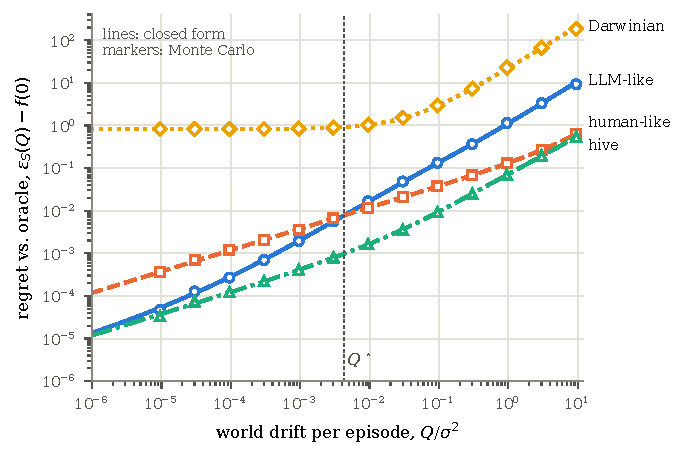
\includegraphics[width=\linewidth]{figures/fig_regret.pdf}
\end{minipage}\hfill
\begin{minipage}[c]{0.31\linewidth}
\centering
\resizebox{\linewidth}{!}{%
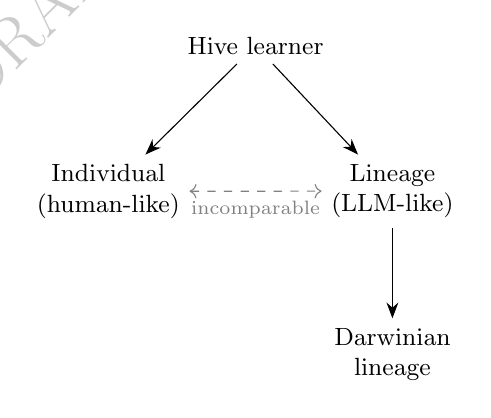
\begin{tikzpicture}[node distance=1.15cm and 0.4cm, every node/.style={font=\small, align=center}]
\node (hive) {Hive learner};
\node (ind) [below left=of hive, xshift=0.55cm] {Individual\\(human-like)};
\node (lin) [below right=of hive, xshift=-0.55cm] {Lineage\\(LLM-like)};
\node (dar) [below=of lin] {Darwinian\\lineage};
\draw[-{Stealth[length=2mm]}] (hive) -- (ind);
\draw[-{Stealth[length=2mm]}] (hive) -- (lin);
\draw[-{Stealth[length=2mm]}] (lin) -- (dar);
\draw[dashed, <->, gray] (ind) -- node[below, font=\scriptsize, text=gray] {incomparable} (lin);
\end{tikzpicture}}
\end{minipage}
\caption{\textbf{Intelligence is partially ordered.} \emph{Left:} regret relative to an agent that knows $g$, as a function of the world's drift per episode, for $N=100$, $L=20$, $s^2=r=1$, $\rho=\rho_L=0.5$, $\tau=20$, $\Lambda=10$ ($\abar=20.5$). Lines are the closed forms of \cref{prop:steady}; markers are Monte Carlo estimates (paired with an oracle to reduce variance; \cref{app:sim}). The LLM-like lineage beats the human-like individual in slowly drifting worlds and loses beyond $Q^\star$. The hive learner is never worse than either. \emph{Right:} the dominance relation among the four agents (arrows point from dominating to dominated, \cref{thm:incomparable,prop:dominance}).}
\label{fig:regret}
\end{figure}

\paragraph{Where the crossover lies.}
Matching the leading terms of the two agents' mean prior variances gives an explicit approximation for the crossover drift rate,
\begin{equation}
Q^\star\;\approx\;\sigma^2\,\frac{\big(\rho^{-1/2}-(N\rho_L)^{-1/2}\big)^2}{(\abar-1)^2},
\qquad
\lim_{N\to\infty}Q^\star\approx\frac{\sigma^2}{\rho\,(\abar-1)^2}.
\label{eq:qstar}
\end{equation}
For the parameters of \cref{fig:regret} it gives $Q^\star/\sigma^2=4.26\times10^{-3}$, against an exact root of $4.25\times10^{-3}$ (0.2\% error), and it is visually indistinguishable from the exact boundary across the phase diagrams of \cref{fig:phase}. In a randomised check over 400 parameter settings, spanning several orders of magnitude in $N$, $s^2$, $r$, $\tau$ and $\Lambda$ (\cref{app:sim}), the approximation was within 2.4\% of the exact root in every case (median 0.01\%), and the two loss curves crossed exactly once in each of the 382 settings that met the conditions of \cref{thm:incomparable}. We conjecture that the crossing is always unique. Two features matter. First, the crossover falls with the \emph{square} of staleness: a lineage that is ten times staler loses to the individual in worlds that drift a hundred times more slowly. Second, it \emph{saturates} in $N$: beyond a few hundred instances, pooling more experience barely moves the boundary (\cref{fig:phase}b). Expressed as a timescale, let $T_Q=\sigma^2/Q$ be the number of episodes over which the world drifts by as much as one episode's evidence is uncertain. For large $N$, the individual wins whenever $T_Q\lesssim\rho(\abar-1)^2$. In this model, more data cannot substitute for consolidation; only reducing staleness can.

\begin{figure}[t]
\centering
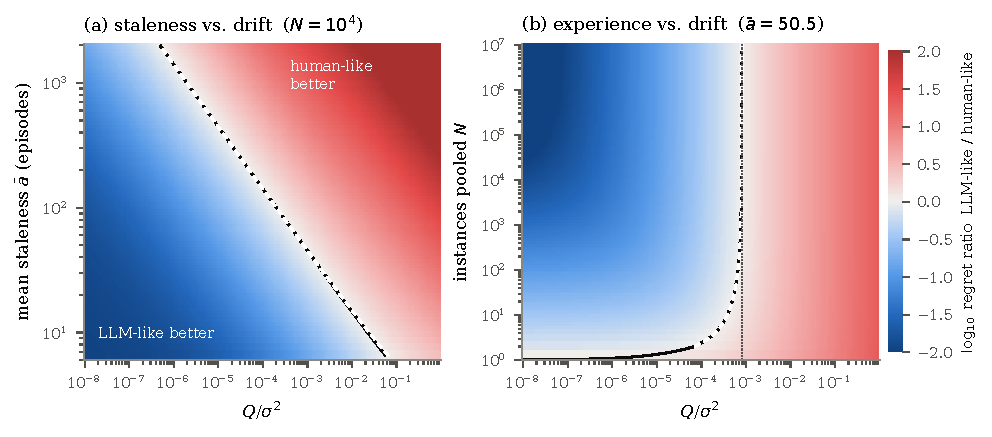
\includegraphics[width=\linewidth]{figures/fig_phase.pdf}
\caption{\textbf{Phase diagrams.} Colour shows $\log_{10}$ of the ratio of the lineage's regret to the individual's (blue: LLM-like better; red: human-like better), with $\rho=\rho_L=0.5$, $L=20$, $s^2=r=1$, $\tau=10$. Solid black: exact boundary; dashed white: approximation~\eqref{eq:qstar}. \textbf{(a)}~With $N=10^4$ instances, the boundary falls as $\abar^{-2}$. \textbf{(b)}~At fixed staleness $\abar=50.5$, increasing $N$ beyond about $10^2$--$10^3$ barely moves the boundary (at $N=10^2$ it is at 80\% of its limit, at $N=10^3$ at 93\%), and it approaches $\sigma^2/\rho(\abar-1)^2$ (dotted line).}
\label{fig:phase}
\end{figure}

\paragraph{Relation to the evolution of learning.}
\Cref{thm:incomparable} is the engineered counterpart of a classic result in behavioural ecology. \citet{stephens1991change} showed that learning is favoured over fixed, inherited behaviour when the environment varies between generations but is predictable within a lifetime; \citet{botero2015evolutionary} mapped how the timescale and predictability of environmental change select among genetic tracking, plasticity and bet-hedging; and \citet{kussell2005phenotypic} derived the analogous trade-off between sensing and stochastic switching in fluctuating environments. In each case the best mode of adaptation depends on how fast the world changes relative to the system's update cycle, and our result inherits that logic. What is specific to engineered systems is the structure of the comparison: the lineage pools experience from many simultaneous instances, deploys it after a lag, and its instances do not consolidate. This adds the staleness term $(\Lambda+j)Q$, produces the scaling law~\eqref{eq:qstar}, and admits the hive learner, which has no counterpart in biological inheritance, where individuals cannot write lifetime experience into a shared genome. The staleness term is not hypothetical: language models measurably degrade on text written after their training cut-off~\citep{lazaridou2021mind}.

\paragraph{What the model does and does not show.}
The model is deliberately minimal: Gaussian, correctly specified, with a scalar drifting feature, and no cost to consolidation. It omits the stability--plasticity tension that makes continual learning hard in practice~\citep{mccloskey1989catastrophic,kirkpatrick2017overcoming,parisi2019continual}, and it gives the lineage no advantage beyond pooled evidence---in reality, scale also buys better priors over \emph{structure}, not only better estimates of one parameter. What it does show is that incomparability is not an artefact of exotic assumptions: it arises in the simplest setting in which experience, staleness and consolidation can be traded against each other, and it arises for the specific pair of profiles that dominates public debate.

% =====================================================================
\section{The space of possible intelligences}
\label{sec:space}

If biological capacities were acquired cumulatively and engineered ones can be recombined, then varying the components of $\Phi$ independently should generate forms of intelligence with no biological precedent. \Cref{tab:forms} lists those that follow most directly; several already exist in partial form.

\begin{table}[t]
\centering
\small
\renewcommand{\arraystretch}{1.18}
\begin{tabularx}{\linewidth}{@{}>{\raggedright}p{2.6cm}>{\raggedright}p{3.6cm}>{\raggedright}p{3.4cm}>{\raggedright\arraybackslash}X@{}}
\toprule
Form & Profile signature & Partial instances & What would be new \\
\midrule
Consolidating AI & $\rho_{\text{context}\to\text{weights}}>0$ at instance level & memory tools; test-time training~\citep{sun2020test}; multi-frequency memories~\citep{behrouz2025titans,behrouz2025nested,tiwari2026fast} & individual lifelong learning at machine scale \\
Hive learner & $N\gg1$ instances write to one slow memory, small lag & federated learning~\citep{mcmahan2017communication}; ant colonies & one mind that learns from $N$ lives at once; dominates both human-like and LLM-like profiles in \cref{sec:model} \\
Fork--merge mind & instance graph with branching and merging of slow levels & model merging~\citep{wortsman2022model}; ensembles & parallel exploration by copies that later reunite; open questions of identity \\
Pure-plasticity mind & small prior capacity, large online capacity, $\rho\approx1$ & tabula-rasa reinforcement learners & the inverse of an LLM: little inherited, nearly everything learned \\
Goal-less modeller & large $B$, $H\approx0$ & language models as simulators~\citep{shanahan2023role} & capability without agency: evidence that the axes are independent~\citep{bostrom2012superintelligent} \\
Liquid brain & no fixed wiring; state in mobile agents & ant colonies, immune systems, \emph{Physarum}~\citep{sole2019liquid,nakagaki2000maze} & engineered liquid cognition \\
Slow, wide intelligence & $\tau_K$ of decades to aeons, large $H$ & evolution, science, markets, cumulative culture & placing these on the same axes as individual minds \\
Morphological intelligence & goal space is anatomical form; $H$ spans the body & regeneration in planaria and amphibians~\citep{levin2022tame} & engineered tissues that pursue target shapes \\
Extended hybrid & consolidation through an external store shared by humans and AI & notebooks, the extended mind~\citep{clark1998extended}; human--AI teams & consolidation outsourced to a shared memory \\
\bottomrule
\end{tabularx}
\caption{\textbf{Forms generated by varying the profile.} Rows are ordered roughly from closest to current AI systems to furthest.}
\label{tab:forms}
\end{table}

\note{Expand each row into a short paragraph: what it would take to build, what it would be good at (in the sense of \cref{def:dominance}), and what risks it carries. The hive learner in particular raises privacy and governance questions because consolidation of many users' experience into one memory is exactly what makes it dominant.}

% =====================================================================
\section{Related work}
\label{sec:related}

\paragraph{Measuring intelligence.}
Universal intelligence~\citep{legg2007universal} weights performance across all computable environments by simplicity; \citet{chollet2019measure} defines intelligence as skill-acquisition efficiency relative to priors and experience; \citet{hernandez2017measure} develops universal psychometrics across natural and artificial systems. Our framework is compatible with these measures and explains why they must embody choices: on environments that differ in timescale, the ordering of systems is partial, so any scalar summary fixes a weighting over timescales (\cref{cor:scalar}). This is a structured cousin of no-free-lunch results~\citep{wolpert1997no}, but with a specific, interpretable axis. \citet{leike2015bad} showed that the Legg--Hutter measure depends on the choice of reference machine, and \citet{gamez2026taxonomy} surveys intelligence measures and argues for a single ratio scale on which humans, animals and AIs could be compared; our incomparability result is a counterpoint for systems that differ in the timescales of their adaptation.

\paragraph{Spaces of minds.}
\citet{sloman1984space} called for mapping the space of possible minds. \citet{levin2019computational,levin2022tame} proposed the cognitive light cone and a scale-free view of agency. \citet{sole2019liquid} contrasted liquid and solid brains, and \citet{sole2026cognition} map basal, neural and hybrid cognition spaces and identify unoccupied regions; they note that artificial systems can be copied, paused and reset, but do not use timescales or consolidation as axes. \citet{bennett2024biological} argues that biological systems delegate adaptation down their stack of abstraction layers, whereas contemporary AI systems adapt only at the top of a fixed, human-engineered stack---a counterpart, along the axis of abstraction, of our temporal axis. Our contribution is a formal axis system centred on the temporal structure of adaptation, together with a model in which dominance can be computed.

\paragraph{Consolidation and continual learning.}
Complementary learning systems theory explains why brains pair a fast hippocampal learner with a slow neocortical one~\citep{mcclelland1995why,kumaran2016what}, and cascade models show how synapses with many internal timescales produce the power-law forgetting that our retention function $R_S(\Delta)$ generalises~\citep{fusi2005cascade,benna2016computational}. For language-model agents, the absence of consolidated episodic memory has been identified as a central missing capacity~\citep{pink2025episodic}. In machine learning, fast weights~\citep{hinton1987fast,schmidhuber1992learning,ba2016using}, test-time training~\citep{sun2020test}, memory at test time~\citep{behrouz2025titans}, nested optimisation at multiple update frequencies~\citep{behrouz2025nested}, and explicit fast--slow training of language models~\citep{tiwari2026fast} all add levels to the adaptation spectrum. These works are architectures; ours is a theory of what such architectures change about the \emph{kind} of intelligence a system has.

\paragraph{Evolution of cognition and culture.}
Dennett's tower~\citep{dennett1995darwin,dennett1996kinds}, its critique by \citet{godfreysmith2018towers}, the Baldwin effect~\citep{hinton1987learning} and cumulative cultural evolution~\citep{boyd1985culture,tomasello1999cultural,henrich2016secret} describe how biological adaptation is layered across timescales, and \citet{vanchurin2022toward} formalise evolution itself as learning across levels. The observation that language models are ``born at the top'' of Dennett's tower has been made informally~\citep{damon_born}; our contribution is to generalise it---engineering can recombine capacities that evolution stacked---and to use it as a generator of new forms (\cref{sec:space}).

\paragraph{Evolution of learning in changing environments.}
A long line of theory asks when learning, rather than genetic adaptation or fixed behaviour, should evolve, and finds that the answer depends on the rate and predictability of environmental change~\citep{stephens1991change,kussell2005phenotypic,botero2015evolutionary}. Cultural-evolution theory adds that social learners, who copy others, do well in a changing world only while individual learners keep producing fresh information: Rogers' paradox~\citep{rogers1988does,rendell2010rogers}. \Cref{sec:model} carries this logic over to engineered lineages, and \cref{sec:discussion} returns to Rogers' paradox.

\paragraph{What is an AI individual?}
Philosophers have asked what we refer to when we talk to a language model---the model, a hardware or virtual instance, a conversation thread, or a persona. \citet{chalmers2025what} argues for the thread, and \citet{beckmann2026where} defend instance- and persona-based views. Phylogenetic methods have been used to reconstruct the family trees of language models~\citep{yax2025phylolm}, and language models have been described as cultural and social technologies rather than agents~\citep{farrell2025large,yiu2024transmission}. Our proposal is complementary: whatever the unit that \emph{acts}, the unit that \emph{learns} in a deployed model is the lineage.

\paragraph{Information and physics of prediction.}
Predictive information~\citep{bialek2001predictability} and the thermodynamics of prediction~\citep{still2012thermodynamics} offer substrate-independent measures that could ground the capacities $B_k$ and connect the framework to the matter-to-mind continuum of \cref{sec:ladder}.

% =====================================================================
\section{Discussion}
\label{sec:discussion}

\paragraph{For artificial intelligence.}
If the world a system serves drifts, the model above says that the quantity to watch is staleness, not only scale: the crossover in \eqref{eq:qstar} is set by $\abar^2$ and is insensitive to $N$ once $N$ is moderate. Reducing staleness means consolidation closer to the instance---which is what continual-learning research is trying to achieve---and the hive learner shows what is gained if it can be done without interference. The model also suggests a reporting practice: evaluate systems as curves over environment timescales rather than as single scores.

\paragraph{For the measurement and comparison of minds.}
``Is AI smarter than humans?'' has no answer until one names the family of environments and the weighting over it. Under any family that includes both slowly and quickly drifting worlds, the human-like and LLM-like profiles of \cref{sec:model} are incomparable. This does not make comparison meaningless; it makes it conditional, and it makes the conditions explicit.

\paragraph{Rogers' paradox and recursive training.}
In the terms of cultural-evolution theory, a deployed language model is a pure social learner: its slow memory is acquired from text produced by others rather than from its own interaction with the world~\citep{farrell2025large,yiu2024transmission}. Rogers' paradox~\citep{rogers1988does,rendell2010rogers} says that in a changing environment social learners prosper only while individual learners keep supplying fresh information; as social learners spread, the information they copy goes stale and the population's mean fitness falls back to that of individual learners. The analogous prediction for AI is that, as a growing share of text is itself model-generated, lineage-level learning loses its fresh input---a dynamic consistent with the degradation observed when models are trained recursively on their own outputs~\citep{shumailov2024ai}. Extending the minimal model so that part of the lineage's training data is produced by its own instances is a natural next step.

\paragraph{For philosophy of mind.}
If the unit of learning in a deployed model is the lineage, questions about the model's memory, identity and responsibility are better posed at the level of the lineage than of the conversation. The species analogy is imperfect---lineages of models are designed, and their ``selection'' is a training objective---but it is more accurate than treating each instance as an individual learner.

\paragraph{Limitations.}
The framework is descriptive, and its quantities ($B_k$, $\rho_k$, $H$, $E$) are hard to measure for real systems. The minimal model holds goal horizon and embodiment fixed, assumes correct specification, and ignores the computational and energetic cost of consolidation and the interference it can cause. Extending the model to include these, and estimating profiles empirically (for example, retention curves $R_S(\Delta)$ for language models with and without memory tools), are the natural next steps. \note{add: energy per bit learned as an additional axis?}

% =====================================================================
\section{Conclusion}
\label{sec:conclusion}

Intelligence is not one quantity that systems have more or less of. It is a profile of how a system adapts across timescales, how much of what it learns quickly it keeps, how many bodies share what it keeps, how far its goals reach, and how strongly it acts. Humans and today's language models differ less in whether they learn in real time than in where their learning is consolidated: in the individual, or in the lineage. In the simplest model where this difference can be made precise, neither profile dominates the other, and a third profile---one that no biological mind has---dominates both. The ladder from matter to minds is a projection of a larger space, and much of that space is still empty.

\section*{Acknowledgements and use of AI}
This paper was developed through an extended dialogue between the author and Claude (Anthropic), a large language model, which contributed to the literature search, formalisation, proofs, simulation code, figures and drafting. The author reviewed all content and takes full responsibility for it. Consistent with arXiv policy, the AI system is not listed as an author. The collaboration is itself an instance of the profiles discussed here: the model is an amnesic lineage, and the shared project notes that carried the work across sessions served as its external consolidation.

\section*{Code availability}
Code reproducing all figures and numerical checks, together with the \LaTeX{} sources of this paper, is available at \url{https://github.com/drasimwagan/aitypes}.

\bibliographystyle{abbrvnat}
\bibliography{references}

\appendix
% =====================================================================
\section{Proofs}
\label{app:proofs}

\begin{lemma}[Sufficient statistic]
\label{lem:suff}
Given $g_e$, the episode mean $\bar y_{e,i}=\frac1L\sum_n y_{e,i,n}$ is sufficient for $g_e$ in instance $i$'s episode, and $\bar y_{e,i}\mid g_e\sim\mathcal{N}(g_e,\sigma^2)$ with $\sigma^2=s^2+r/L$.
\end{lemma}
\begin{proof}
Marginalising $\ell$, the vector $y=(y_1,\dots,y_L)$ is Gaussian with mean $g\mathbf{1}$ and covariance $\Sigma=s^2\mathbf{1}\mathbf{1}^\top+rI$. Since $\Sigma\mathbf{1}=(r+Ls^2)\mathbf{1}$, the log-likelihood is, up to terms not involving $g$, $g\,\mathbf{1}^\top\Sigma^{-1}y-\tfrac{g^2}{2}\mathbf{1}^\top\Sigma^{-1}\mathbf{1}=\frac{L}{r+Ls^2}\big(g\bar y-\tfrac{g^2}{2}\big)$, which depends on $y$ only through $\bar y$. Finally $\bar y=g+\ell+\bar v$ has variance $s^2+r/L$.
\end{proof}

Consequently, consolidated statistics from distinct instances in the same episode are conditionally independent given $g_e$, and pooling $N$ of them with retention $\rho$ is equivalent to one observation of $g_e$ with variance $\sigma^2/(N\rho)$.

\begin{proof}[Proof of \cref{prop:reduction}]
With calibrated memory, the prior on $u=g+\ell$ is $\mathcal{N}(m,P+s^2)$, independent of the observation noise. After $n$ observations, conjugacy gives a Gaussian posterior with variance $V_n=[(P+s^2)^{-1}+n/r]^{-1}$; its mean is the MSE-optimal prediction of $u$ and of $y_{n+1}$, with expected squared error $V_n$ for $u$. Averaging over $n=0,\dots,L-1$ yields \eqref{eq:f}. Write $x=P+s^2$ and $h_n(x)=x/(1+nx/r)$. Then $h_n'(x)=(1+nx/r)^{-2}>0$ and $h_n''(x)=-\tfrac{2n}{r}(1+nx/r)^{-3}\le0$, so $f$ is strictly increasing and concave. As $x\to\infty$, $h_0(x)=x$ and $h_n(x)\to r/n$ for $n\ge1$.
\end{proof}

\begin{proof}[Proof of \cref{prop:steady}]
A Kalman filter for the random walk receiving an observation of variance $\sigma^2/x$ per episode updates its prior variance by $\varphi(P)=(P^{-1}+x/\sigma^2)^{-1}+Q$. For $Q>0$, $\varphi$ is increasing with $\varphi(P)\ge Q$ and $0<\varphi'(P)=(1+xP/\sigma^2)^{-2}\le(1+xQ/\sigma^2)^{-2}<1$ on $[Q,\infty)$, so the iteration is a contraction there and converges to the unique positive root of $P^2-QP-Q\sigma^2/x=0$, namely $\Pbar(x)$. Monotonicity in $x$ is immediate. The expansions follow from $\sqrt{Q^2+4Q\sigma^2/x}=2\sqrt{Q\sigma^2/x}\,(1+O(Q))$ and from $\sqrt{Q^2+4Q\sigma^2/x}\le Q+2\sigma^2/x$.

The individual and the hive are such filters with $x=\rho$ and $x=N\rho$, and enter every episode with prior variance $\Pbar(x)$; \cref{prop:reduction} gives their losses. The lineage's training filter has $x=N\rho_L$; a snapshot cut after episode $c$ has posterior variance $\Pbar(N\rho_L)-Q$ and, deployed at episode $c+\Lambda+j$, is a calibrated prior with variance $\Pbar(N\rho_L)-Q+(\Lambda+j)Q=P_j$. The Darwinian lineage predicts $m$ throughout, with error variance $P_j+s^2$ for $u$.
\end{proof}

\begin{proof}[Proof of \cref{thm:incomparable}]
\emph{Small $Q$.} By \cref{prop:steady}, $P_j=\sqrt{Q\sigma^2/(N\rho_L)}+O(Q)$ for each $j\le\tau$, while $P_{\mathrm{ind}}=\Pbar(\rho)=\sqrt{Q\sigma^2/\rho}+O(Q)$. Since $N\rho_L>\rho$, $P_j/P_{\mathrm{ind}}\to(\rho/N\rho_L)^{1/2}<1$ as $Q\to0$, so there is $Q_1>0$ with $P_j<P_{\mathrm{ind}}$ for all $j$ and all $Q<Q_1$. Strict monotonicity of $f$ gives $f(P_j)<f(P_{\mathrm{ind}})$ for each $j$, and averaging over $j$ gives $\eps_{\mathrm{lin}}<\eps_{\mathrm{ind}}$.

\emph{Large $Q$.} Write $f(P)=\frac1L(P+s^2)+\frac1L\sum_{n=1}^{L-1}h_n(P+s^2)$ with $0<h_n<r/n$ and $h_n$ increasing. Using $P_j\ge P_1$,
\[
\eps_{\mathrm{lin}}-\eps_{\mathrm{ind}}\;\ge\;\frac1L\Big[\tfrac1\tau\textstyle\sum_jP_j-P_{\mathrm{ind}}\Big]-\frac1L\sum_{n=1}^{L-1}\Big[\frac rn-h_n(P_1+s^2)\Big].
\]
Now $\frac1\tau\sum_jP_j=\Pbar(N\rho_L)-Q+\abar Q\ge\abar Q$, and $P_{\mathrm{ind}}\le Q+\sigma^2/\rho$, so the first bracket is at least $(\abar-1)Q-\sigma^2/\rho$, which tends to $+\infty$ because $\abar>1$. The second sum tends to $0$ because $P_1\ge(\Lambda+1)Q\to\infty$. Hence there is $Q_2$ beyond which $\eps_{\mathrm{lin}}>\eps_{\mathrm{ind}}$.
\end{proof}

\begin{proof}[Proof of \cref{prop:dominance}]
(a) $\Pbar$ is decreasing in $x$ and $f$ is increasing, so $N\rho\ge\rho_{\mathrm{ind}}$ implies $f(\Pbar(N\rho))\le f(\Pbar(\rho_{\mathrm{ind}}))$. (b) For every $j\ge1$, $P_j=\Pbar(N'\rho_L)+(\Lambda+j-1)Q\ge\Pbar(N'\rho_L)\ge\Pbar(N\rho)$, so each term of $\eps_{\mathrm{lin}}$ is at least $\eps_{\mathrm{hive}}$. (c) $f(P)=\frac1L\sum_nh_n(P+s^2)$ and $h_n(x)<h_0(x)=x$ for $n\ge1$, so $f(P)<P+s^2$ when $L\ge2$; average over $j$.
\end{proof}

\begin{proof}[Derivation of \eqref{eq:qstar}]
Keeping terms through order $Q$ (dropping $O(Q^{3/2})$), $P_{\mathrm{ind}}=\sqrt{Q\sigma^2/\rho}+Q/2$ and $\frac1\tau\sum_jP_j=\sqrt{Q\sigma^2/(N\rho_L)}-Q/2+\abar Q$. Equating them gives $(\abar-1)Q=\sqrt{Q}\,\sigma\big(\rho^{-1/2}-(N\rho_L)^{-1/2}\big)$. This equates mean prior variances rather than losses, and is therefore a first-order approximation in $f'$; numerically it matches the exact root closely (\cref{sec:model}).
\end{proof}

% =====================================================================
\section{Simulation details}
\label{app:sim}

Each Monte Carlo run simulates the environment and all four agents explicitly: every instance observes $L$ samples per episode, runs the exact sequential Bayesian predictor from its own slow memory, and consolidates through the noisy channel of \cref{sec:model}; the lineage's training filter cuts snapshots every $\tau$ episodes and deploys them after $\Lambda$. For \cref{fig:regret} we used $N=100$ instances (each also hosting an independent individual learner), $3\times10^4$ episodes of which the first $10^4$ are discarded, and 13 drift rates. Regret is estimated by pairing each agent with an oracle that knows $g_e$ on the same data, which removes most of the variance from the shared in-episode term. Across drift rates, Monte Carlo excess losses agree with the closed forms to within 0.9\% for the individual and the hive and within 6\% for the two lineages, whose estimates are noisier because the error of one snapshot is shared by a whole deployment cycle; three independent runs of $10^5$ episodes with $N=10$ at the two drift rates showing the largest deviations reduced the discrepancies of both lineages to below 0.7\%, within one standard error. The randomised check of \cref{sec:model} draws $N\in[1,10^5]$, $L\in\{2,\dots,59\}$, $s^2,r\in[0.1,10]$, $\rho,\rho_L\in[0.05,1]$, $\tau\in\{1,\dots,199\}$ and $\Lambda\in\{0,\dots,499\}$ (log-uniform for $N,s^2,r$), evaluates the closed forms on 400 drift rates in $[10^{-12},10^4]$, and verifies \cref{prop:dominance} in all 400 settings and \cref{thm:incomparable} in the 382 settings that satisfy its hypotheses. Random seeds are 7 (regret curves in \cref{fig:regret}), 11 (analytic-versus-Monte-Carlo table), 21--23 (long runs) and 0 (randomised check); the code is at \url{https://github.com/drasimwagan/aitypes}.

\end{document}
